\begin{longtable} { | c | p{12cm} | c | } 
\hline
	ID 	&	Issues	&		 Es. hours \\\hline
	 65	&	Sequenceviewer: Play/Pause/Stop sound	&	32 hours \\\hline
\caption{Issue ID 65}
\label{tab:spr4_SVplaypausestopsound}
\end{longtable}

This issue comes from the general specification requirements, see appendix \ref{app:reqgroup1}. Additionally, it is a requirement from the Parrot-group to be able to play sound, otherwise their application would not have any use of Sequenceviewer.

The functionality for playing sound has already been developed by the Parrot-group together with the PictoCreator-group. They created a library in the pictogram-lib project, which holds the functionality. Therefore, Sequenceviewer uses this library to play and stop sound. There was no request from the customers for pause, neither did any of the other two groups implement the functionality.

To use the library, we implemented three methods: \ct{onClickPlaySound(), playNext(), and soundDonePlaying()}. We use a list of byte-array to hold the sound for each pictogram in a sequence. That makes it possible to iterate over the pictograms in a sequence, and display they attached sound accordingly. This happens by instantiating a version of a PictoMediaPlayer from the pictogram-lib, as well as implementing the CompleteListener, which tells the PictoMediaPlayer when a pictogram is done playing the attached sound. These initiating parts can be seen in listing \ref{lst:pictomediaplayer}.

\begin{lstlisting} [caption={Instantiating the PictoMediaPlayer from pictogram-lib}, label={lst:pictomediaplayer}]
import dk.aau.cs.giraf.pictogram.PictoMediaPlayer;

public class HorizontallyScroll extends GHorizontalScrollViewSnapper implements CompleteListener{
...
PictoMediaPlayer pictoMediaPlayer = new PictoMediaPlayer(getContext());
...
}
\end{lstlisting}

We start off by setting up buttons for playing and stopping sound. This is done in a method called \ct{setupSoundButtons()}. We defined buttons for playing and stopping sound in the landscape$\_$mode.xml-file, and we now set their visibility to \textit{visible}. We attach an \ct{onClickListener} to each of the buttons, and add functionality for playing sound and stopping sound. The code for the \ct{onClickListener} can be see in listing \ref{lst:soundonClickListeners}.

\begin{lstlisting} [caption={onClickListeners for playSound() and stopSound()}, label={lst:soundonClickListeners}]
        playButton.setOnClickListener(new OnClickListener() {
            @Override
            public void onClick(View v) {
                try {
                   onClickPlaySound();
                    index = 0;
                }
                catch(Exception e) {

                }
            }
        });

        stopButton.setOnClickListener(new OnClickListener() {

            @Override
            public void onClick(View v) {
                pictoMediaPlayer.stopSound();
                index = 0;
            }
        });
\end{lstlisting}

Now the pictoMediaPlayer goes through the sequence and playing the sound attached to the pictogram. This happens by initiating the playSound by starting \ct{onClickPlaySound()}, which sets the customListener to the current pictoMediaPlayer. It then calls \ct{playNext}, which set the datasource of the pictoMediaPlayer to be the first sound-element to be played in \ct{soundToPlay}. It plays the sound and increments the index pointer. Once the sound is done playing, \ct{soundDonePlaying} calls \ct{playNext()} again, and if the index within the number of \ct{soundToPlay} it continues, until this does not hold. The code for these three methods can be seen in listing \ref{lst:soundplaymethods}.

\begin{lstlisting} [caption={The three methods associated with playing sound in Sequenceviewer}, label={lst:soundplaymethods}]
    private void playNext(){
        if(index < soundToPlay.size()){
            pictoMediaPlayer.setDataSource(soundToPlay.get(index));
            pictoMediaPlayer.playSound();
            index++;
        }
    }

    private void onClickPlaySound(){
        pictoMediaPlayer.setCustomListener(this);
        playNext();

    }

    @Override
    public void soundDonePlaying() {
        playNext();
    }
\end{lstlisting}

Figure \ref{fig:soundBtns} shows a sequence with sound attached to the pictograms. The sound can be played by clicking the play-button. The sound can be stopped by pressing the stop-button.

\begin{figure}[H]
	\centering
	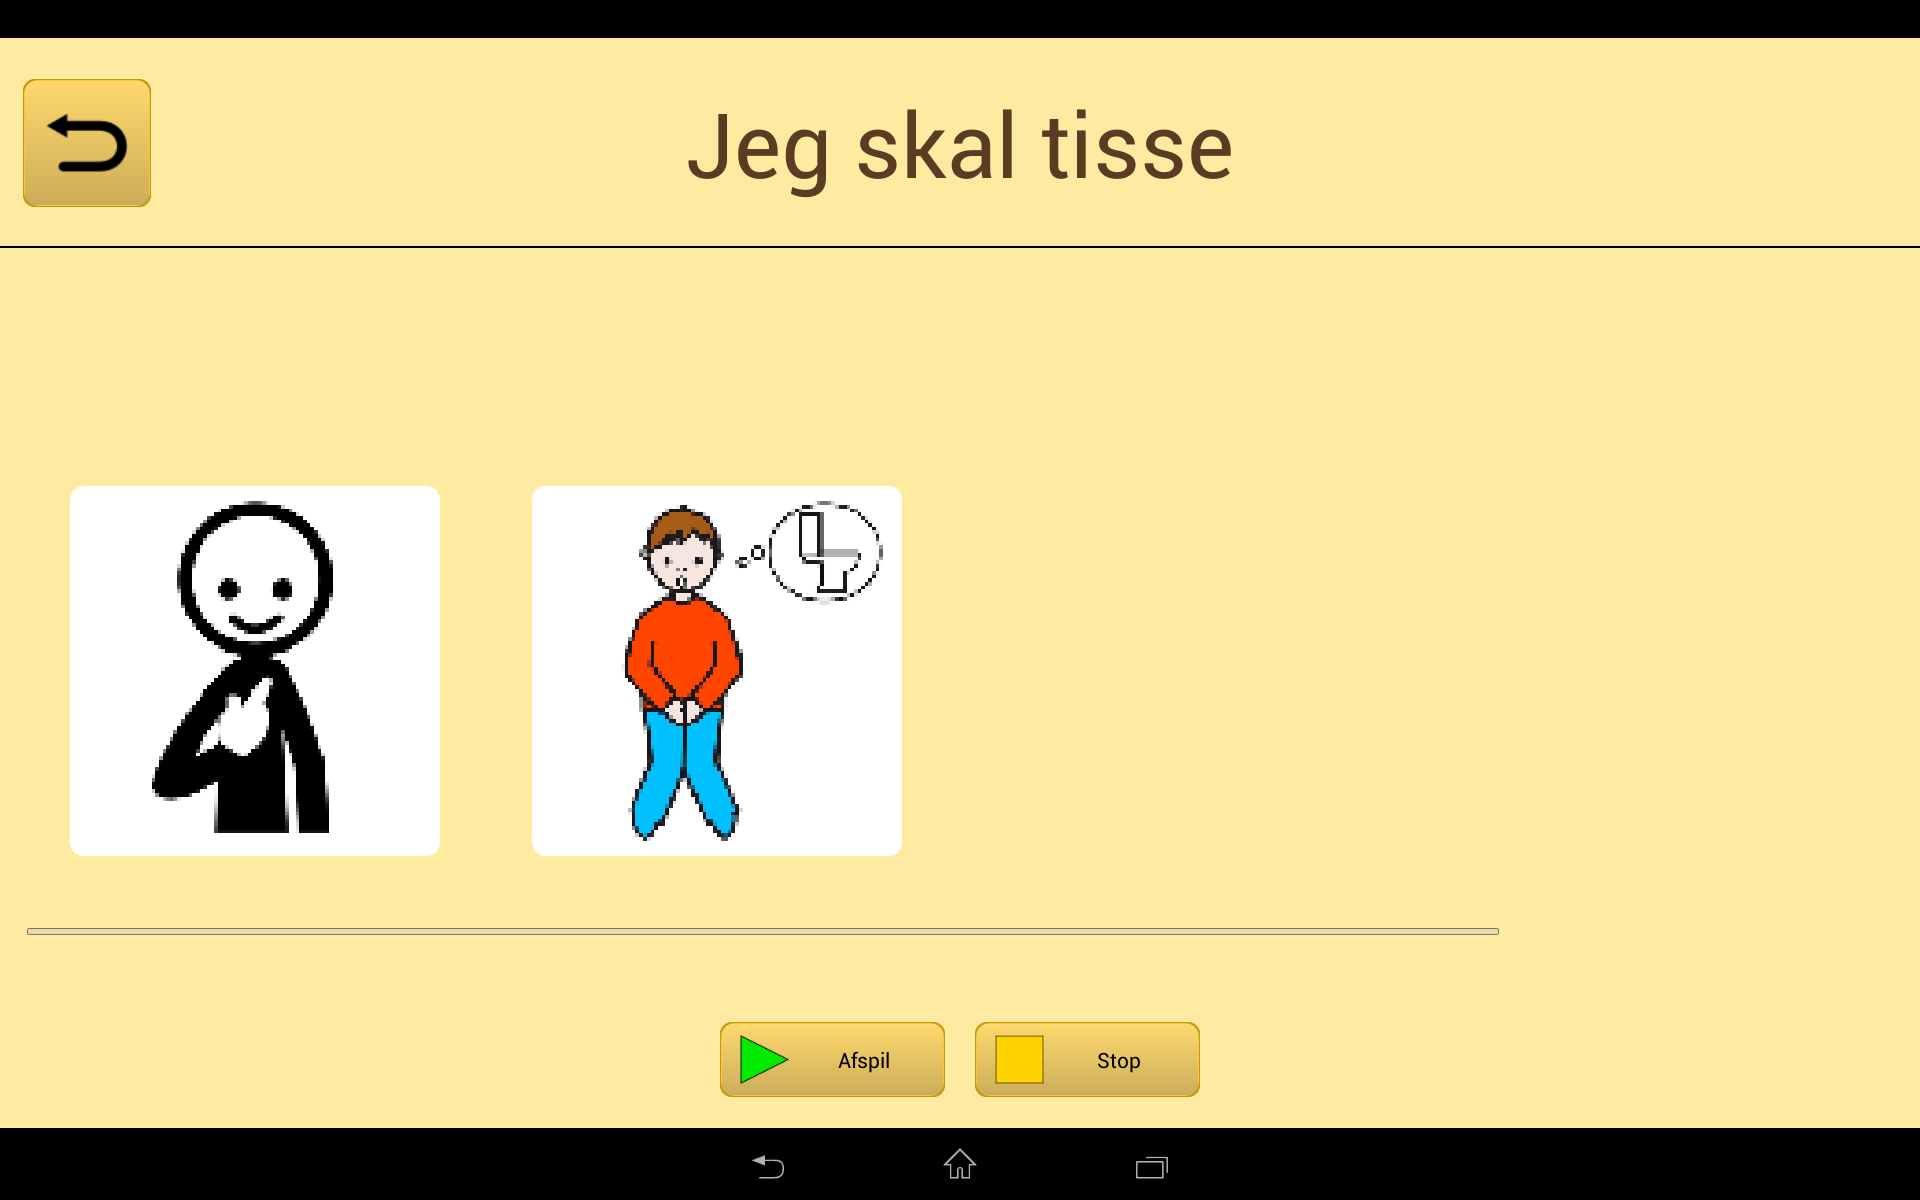
\includegraphics[scale=0.15]{Pics/Sprint4/soundbuttons.png}
	\caption{A sequence with the possibility to play and stop sound. }
	\label{fig:soundBtns}
\end{figure}
